\chapter{Quantum Optimal Control Theory} \label{chap:OptimalControl}
The fundamental problem of Quantum Optimal Control Theory is to steer the dynamics of a quantum system in a desired way through external fields \cite{Rice2000,Shapiro2003}. Often, the goal is the transfer from an initial state, $\ket{\psi_0}$, to a desired target-state, $\ket{\psi_{\mathrm{target}}}$. The fields responsible for controlling the dynamics of the system are parametrized by a set of control parameters or functions. Optimal control theory determines the parameters, which lead to the desired dynamics of the system \cite{Werschnik2007}.\\ 
In control problems, the Hamiltonian of the system is given as
\begin{equation}
	\hat{H} =  \hat{H}_0 + \sum_{n = 1}^{m}  \hat{H}_n (u_n(t)) \; ,
	\label{eq:ControlHamiltonians}
\end{equation} 
where $\hat{H}_0$ is an uncontrollable drift, $\hat{H}_n$ are the controllable fields, and $u_n(t)$ are the control functions.

The control problem presented in this thesis is steering the system from an initial state in the superfluid phase to a target-state in the Mott-Insulator phase. This is achieved by varying the lattice depth, which therefore can be considered the control parameter. The optimal control problem can be stated as follows:\\
Suppose the system is initially described by the state $\ket{\psi_0} = \ket{\psi (0)}$, and the potential is varied in the time interval $[ 0 , T]$. The goal is finding the set of control parameters, $\boldsymbol{u}(t)$, which brings the initial state as close as possible to the target-state, $\ket{\psi_{\mathrm{target}}}$. This is expressed in terms of a cost function
\begin{equation}
	\mathcal{J}_T = \frac{1}{2} \left( 1-|\braket{\psi_{\mathrm{target}} | \psi (T)}|^2 \right) \; ,
	\label{eq:infidelityCost}
\end{equation}
which is given as half the infidelity between the target and the state at $t=T$. The cost function becomes zero, when the terminal state matches the target state up to an arbitrary phase. Hence, the optimal control problem can be formulated as a minimization problem of eq. \eqref{eq:infidelityCost} , whereby one can employ methods from mathematical optimization theory \cite{Jager2014}.\\
Large variations in the control parameter is often hard to achieve experimentally. Therefore, an extra term is added to the cost function, which penalizes strong variations in the control. The new cost function reads
\begin{equation}
	\mathcal{J} = \mathcal{J}_T + \mathcal{J}_R = \mathcal{J}_T + \frac{\gamma}{2} \sum_{n=1}^{m} \int_{0}^{T} \left( \pdv{u_n}{t} \right)^2 \mathrm{d}t \; ,
	\label{eq:grapeCost}
\end{equation}
where $\gamma$ weighs the relative importance between matching states and smoothness of the control \cite{Jager2014}. As the state transfer is considered the highest priority, $\gamma \ll 1$ such that $\mathcal{J}_T$ dominates the cost function of eq. \eqref{eq:grapeCost}.


\section{The Gradient-Ascent Pulse Engineering Method - GRAPE} \label{sec:GRAPE}
A powerful way of performing optimal control is the Gradient-Ascent Pulse Engineering (GRAPE) method. Through GRAPE, the gradient of the cost function \eqref{eq:grapeCost} can be evaluated and used to update the existing set of controls \cite{Khaneja2005}. Thereby, one achieves an optimization of the cost function \eqref{eq:grapeCost}.

The gradient of the cost function can be derived in multiple ways. A common method is introducing a Lagrange multiplier \cite{Hohenester2007, Winckel2008, BECcontrol}, which forces the dynamics to obey the Schrödinger equations. This method considers the states and the control as continuous functions, which must be discretized after the derivation of the gradient for numerical purposes. However, postponing the discretization until the very last step causes a loss of accuracy, as a series of higher order corrections due to the discretization are lost.
Here, an alternative derivation following \cite{Khaneja2005, deFouquieres2011} is presented in which the discretization is introduced immediately. \\
Assume the transfer time, $T$, is discretized in steps of $\Delta t = T/N$. Subjecting the control to a similar discretized yields
\begin{equation}
	u_n = \left( u_n (t_1) , \ldots , u_n (t_N)  \right)  \; .
\end{equation}
The time-evolution of the system during the time step $j$ is given by the propagator
\begin{equation}
	\hat{\mathcal{U}}_j \equiv \hat{\mathcal{U}} (u(t_j)) = \exp \bigg\{ -i \left( \hat{H}_0  \sum_{n = 1}^{m}  \hat{H}_n (u_n(t_j))  \right) \Delta t \bigg\} \; . 
\end{equation} 
Thereby, the cost function \eqref{eq:grapeCost} becomes
\begin{equation}
	\mathcal{J} = \frac{1}{2} \left( 1 - |\braket{\psi_{\mathrm{target}} | \prod_{j = 1}^{N} \hat{\mathcal{U}}_j | \psi (0)}|^2 \right) + \frac{\gamma}{2} \sum_{n = 1}^{m} \sum_{j = 1}^{N-1} \left( \frac{\Delta u_n (t_j)}{\Delta t} \right)^2 \Delta t \; ,
	\label{eq:discreteCost}
\end{equation}
where $\Delta u_n (t_j) =  u_n (t_{j+1}) - u_n (t_j)$. The full gradient of the cost, $\nabla \mathcal{J}(\boldsymbol{u})$, is a vector of partial derivatives ${\partial \mathcal{J}(\boldsymbol{u})}/{\partial u_n (t_j)}$, which can be derived analytically.\\
First, consider the derivative of the regularization
\begin{align}
	\frac{\partial \mathcal{J}_R}{\partial u_n (t_j)} &= \frac{\gamma}{2} \left( 2 \frac{u_n (t_j) - u_n (t_{j-1})}{\Delta t^2} - 2 \frac{u_n (t_{j+1}) - u_n (t_j)}{\Delta t^2} \right) \Delta t \nonumber \\
	&= \frac{\gamma}{\Delta t} \left( 2 u_n (t_j) - u_n (t_{j+1}) - u_n (t_{j-1}) \right) \; . \label{eq:regularizationGrad}
\end{align}
The part of the gradient related to the regularization depends only on the control, whereby it can be calculated without considering the state of the system.\\ 
Next, consider the derivative of $\mathcal{J}_T$. Defining the transfer probability amplitude $\mathcal{T} \equiv \braket{\psi_{\mathrm{target}} | \psi (T)}$, the derivative of the final infidelity with respect to the control can be written as 
\begin{equation}
	\frac{\partial \mathcal{J}_T}{\partial u_n (t_j)} = - \frac{1}{2} \frac{\partial}{\partial u_n (t_j)}  \mathcal{T}^* \mathcal{T}   = - \Re \left( \mathcal{T}^* \frac{\partial \mathcal{T}}{\partial u_n (t_j)} \right) \; .
	\label{eq:dJTdu}
\end{equation}
From eq. \eqref{eq:dJTdu} it is evident that the derivative of the infidelity depends only on the derivative of the transfer probability amplitude, ${\partial \mathcal{T}}/{\partial u_n (t_j)}$. This derivative can be rewritten as
\begin{align}
	\frac{\partial \mathcal{T}}{\partial u_n (t_j)} &= \frac{\partial }{\partial u_n (t_j)} \Braket{\psi_{\mathrm{target}} | \prod_{j = 1}^{N} \hat{\mathcal{U}}_j | \psi (0)} \nonumber \\
	&= \Braket{\psi_{\mathrm{target}} | \hat{\mathcal{U}}_N \ldots \hat{\mathcal{U}}_{j+1} \frac{\partial \hat{\mathcal{U}}_{j}}{\partial u_n (t_j)} \hat{\mathcal{U}}_{j-1} \ldots \hat{\mathcal{U}}_{1} | \psi (0)}
	\label{eq:dcdu}
\end{align}
Multiplying eq. \eqref{eq:dcdu} with $\mathcal{T}^*$ yields
\begin{align}
	\mathcal{T}^* \frac{\partial \mathcal{T}}{\partial u_n (t_j)} &=  \braket{\psi(T) | \psi_{\mathrm{target}}} \Braket{\psi_{\mathrm{target}} | \prod_{j' = j +1}^{N} \hat{\mathcal{U}}_{j '} \frac{\partial \hat{\mathcal{U}}_{j}}{\partial u_n (t_j)} \prod_{j' = 1}^{ j-1} \hat{\mathcal{U}}_{j '} | \psi (0)} \\
	&= i \Braket{\chi (T) | \prod_{j' = j +1}^{N} \hat{\mathcal{U}}_{j '} \frac{\partial \hat{\mathcal{U}}_{j}}{\partial u_n (t_j)} \prod_{j' = 1}^{ j-1} \hat{\mathcal{U}}_{j '} | \psi (0)} \\
	&= i \Braket{\chi (t_j) |  \frac{\partial \hat{\mathcal{U}}_{j}}{\partial u_n (t_j)} | \psi (t_{j-1})} \; ,
	\label{eq:TaudTau}
\end{align}
where $\ket{\chi (T)} \equiv i \ket{\psi_{\mathrm{target}}} \braket{\psi_{\mathrm{target}} | \psi (T)}$ is the projection of the final state unto the target state. Notice how in eq. \eqref{eq:gradientForBack} the state $\ket{\chi (T)}$ has been propagated backwards in time. Finally, inserting eq. \eqref{eq:TaudTau} into the derivative of the transfer cost function \eqref{eq:dJTdu} produces
\begin{equation}
	\frac{\partial \mathcal{J}_T}{\partial u_n (t_j)} = - \Re \Braket{\chi (t_j) | i \frac{ \partial \hat{\mathcal{U}}_{j}}{\partial u_n (t_j)} | \psi (t_{j-1})} \; .
	\label{eq:gradientForBack}
\end{equation}
The derivative of the propagator, $\hat{\mathcal{U}}_{j}$, is non-trivial, due to possible non-commutativity between the Hamiltonian and its derivative. This results in a series of higher order corrections to the derivative of propagator.
Expanding the propagator as a Taylor series before taking the derivative gives
\begin{align}
	\frac{\partial \hat{\mathcal{U}}_{j}}{\partial u_n (t_j)} &= \frac{\partial}{\partial u_n (t_j)}  \exp \left( -i \hat{H} \Delta t \right) \nonumber \\
	&= \sum_{p = 0}^{\infty} \frac{( -i \Delta t  )^p}{p!} \frac{\partial \hat{H}^p}{\partial u_n (t_j)} \; .  
	\label{eq:derivTaylorExp}
\end{align}
As mentioned before the Hamiltonian may not commute with its derivative. Therefore, one must be careful when taking the derivative of $\hat{H}^p$. Retaining the ordering of the operators while taking the derivative yields
\begin{align}
	\frac{\partial \hat{\mathcal{U}}_{j}}{\partial u_n (t_j)} &= \sum_{p=1}^{\infty} \frac{ \left( -i \Delta t \right) ^p }{p!} \sum_{q=0}^{p-1} \hat{H}^q \frac{\partial \hat{H}}{\partial u_n (j)} \hat{H}^{p-q-1} \nonumber \\
	&= \sum_{p=0}^{\infty} \sum_{q=0}^{\infty} \frac{A^p B A^q}{(p+q+1)!} \; , \label{eq:derivTaylorExp2}
\end{align} 
where $A \equiv -i \hat{H} \Delta t$ and $B \equiv -i \partial \hat{H}/\partial u_n (t_j) \Delta t$ have been defined for notational convenience. Through the standard relations of the gamma function, $\Gamma (z)$, one can derive the identity
\begin{equation}
	\frac{1}{(p+q+1)!} = \frac{1}{p! q !} \int_{0}^{1} (1-\alpha)^p \alpha^q \mathrm{d}\alpha \; .
\end{equation}
Thereby eq. \eqref{eq:derivTaylorExp2} can be expressed as
\begin{align}
	\frac{\partial \hat{\mathcal{U}}_{j}}{\partial u_n (t_j)} &= \sum_{p=0}^{\infty} \sum_{q=0}^{\infty} \frac{A^p B A^q}{p! q !}  \int_{0}^{1} (1-\alpha)^p \alpha^q \mathrm{d}\alpha \nonumber \\
	&= \int_{0}^{1} \sum_{p=0}^{\infty} \sum_{q=0}^{\infty} \frac{(A (1- \alpha))^p}{p!} B \frac{(A \alpha)^q}{q!}  \mathrm{d}\alpha \nonumber \\
	&= \int_{0}^{1} e^{ (1- \alpha) A} B e^{ \alpha A} \mathrm{d}\alpha \nonumber \\
	 &= e^A \int_{0}^{1} e^{ - \alpha A} B e^{ \alpha A} \mathrm{d}\alpha \; , \label{eq:eq:derivTaylorExp3}
\end{align}
where the expansion of the exponential function has been used to eliminate the sums. Although eq. \eqref{eq:eq:derivTaylorExp3} looks rather simple, evaluating the integral in its current form is a fairly hard task. Instead, the integral can be explicitly solved by applying the Baker–Campbell–Hausdorff expansion 
\begin{equation}
	e^X Y e^{-X} = \sum_{k = 0}^{\infty} \frac{ [ X,Y  ]_k }{k!} = Y + [ X,Y  ] + \frac{1}{2!} [ X , [ X,Y  ]] + \frac{1}{3!} [X, [ X , [ X,Y  ]]  ] + ...
\end{equation}
where $[ X , Y ]_k = [ X ,[ X , Y]]_{k-1}$ and $[X,Y]_0 = Y$ is the definition of the recursive commutator \cite{Wilcox1967}. Thus, eq. \eqref{eq:eq:derivTaylorExp3} reads
\begin{align}
	\frac{\partial \hat{\mathcal{U}}_{j}}{\partial u_n (t_j)} &=  e^A \int_{0}^{1} \sum_{k = 0}^{\infty } \alpha^{k} \frac{(-1)^k}{k!} [ A,B  ]_k \mathrm{d}\alpha \nonumber \\
	&= e^A  \sum_{k = 0}^{\infty }  \frac{(-1)^k}{(k+1)!} [ A,B  ]_k \; .
\end{align}
Inserting this final expression for the derivative of the propagator into eq. \eqref{eq:dJTdu}, one finds the exact derivative of the infidelity 
\begin{align}
\frac{\partial \mathcal{J}_T}{\partial u_n (t_j)} &=  - \Re  \Braket{\chi (t_j) | i e^{-i \hat{H} \Delta t}  \sum_{k = 0}^{\infty }  \frac{(-1)^k}{(k+1)!} \left[ -i \hat{H} \Delta t , -i \frac{\partial \hat{H}}{\partial u_n (t_j)} \Delta t  \right]_k | \psi (t_{j-1})}  \nonumber \\
	&=  - \Re  \Braket{\chi (t_{j-1}) | \sum_{k = 0}^{\infty }  \frac{i^{k} \Delta t^{k+1}}{(k+1)!} \left[ \hat{H} , \frac{\partial \hat{H}}{\partial u_n (t_j)}  \right]_k | \psi (t_{j-1})}  \; . \label{eq:higherOrderGradient}
\end{align}
For small time-steps the higher order corrections can be neglected, however, choosing a larger time-step reduces the run-time of the time-evolution, which is critical when describing many-body systems. Therefore, when using large time-steps, higher-order correlations should be included to preserve accuracy. Computing the higher order corrections can be done efficiently by analytically deriving the commutators beforehand. In section \ref{sec:modTMDRG} an alternative propagator is constructed using the Suzuki-Trotter expansion, which causes the gradient to be exact to zeroth order.\\
Finally, combining the derivatives of eq. \eqref{eq:regularizationGrad} and \eqref{eq:higherOrderGradient} produces the entries of the gradient vector for the cost function
\begin{align}
	\frac{\partial \mathcal{J} (\boldsymbol{u})}{\partial u_n (t_j)}  &= - \Re \Braket{\chi (t_{j-1}) | \left( i \frac{\partial \hat{H}}{\partial u_n (t_j)} \Delta t + \mathrm{h.o.} \right)  | \psi (t_{j-1})}  \nonumber \\
	& \quad + \frac{\gamma}{\Delta t} \left( 2 u_n (t_j) - u_n (t_{j+1}) - u_n (t_{j-1}) \right) \; .
	\label{eq:costGradient}
\end{align}
Here $\mathrm{h.o.}$ denotes all higher order terms ($k > 0$).\\ 
Through the analytically derived gradient, the cost can be iteratively updated using gradient-based optimization methods until a desired threshold is reached. This forms the framework of the Gradient-Ascent Pulse Engineering (GRAPE) algorithm \cite{Khaneja2005}.
\begin{algorithm}
\begin{algorithmic}
\caption{GRAPE Algorithm}
\State Choose initial control $\boldsymbol{u}^{(1)}$.
\While{$ \mathcal{J} > \mathcal{J}_{\mathrm{threshold}}$}
	\State Calculate $\ket{\psi (t_k)} = \prod_{j=1}^{k} \hat{\mathcal{U}}_j \ket{\psi (0)}$ for $k = 1 \ldots N$.
	\State Calculate $\ket{\chi (t_k)} = \prod_{j=N}^{k} \hat{\mathcal{U}}_{j}^{\dag} \ket{\chi (T)}$ for $k = N \ldots 1$. 
	\State Evaluate $\frac{\partial \mathcal{J}}{\partial u_n (t_k)}$ for $k = 1 \ldots N$ and $n = 1 \ldots m$ according to eq. \eqref{eq:costGradient}.
	\State Update controls using gradient such that $J^{(i + 1)} < J^{(i)}$. 
\EndWhile
\end{algorithmic}
\end{algorithm}
The cost is minimized under the initial and terminal condition
\begin{align}
	\boldsymbol{u}(0) &= \text{fixed value} \label{eq:firstBound} \\
	\boldsymbol{u}(T) &= \text{fixed value} \\
	\ket{\psi (0)} &= \ket{\psi_0} \\
	\ket{\chi (T)} &= i \ket{\psi_{\mathrm{target}}} \braket{\psi_{\mathrm{target}} | \psi (T)} \; .  \label{eq:lastBound}
\end{align}
Although the starting guess of the control, $\boldsymbol{u}^{(1)}$, can be completely random, both faster convergence and lower convergence value is achieved by choosing a good starting seed. Clearly, there is no guarantee that the algorithm will converge to the global optimum, as it is based on a gradient ascent procedure \cite{Khaneja2005}. Nevertheless, the algorithm can be made to search a large portion of the parameter space by executing it multiple time for various seeds.  

In practice, the GRAPE algorithm requires a lot of computer memory, as the gradient of the cost requires the inner product of the states $\ket{\psi}$ and $\ket{\chi}$ at all times, $t_k$. The two states cannot be time-evolved simultaneously, as $\ket{\chi}$ is derived from the final state. To efficiently evaluate the gradient, the state $\ket{\psi}$ must be stored at each time-step, while entries of the gradient \eqref{eq:costGradient} are calculated at each step of the back-propagation of $\ket{\chi}$. Thus, a total of $N$ states must be kept in each iteration of the GRAPE algorithm. For complex many-body systems this may become an issue, as tensor-network descriptions of states (described in chapter \ref{chap:MPS}) require a lot of storage. A possible workaround is proposed in \cite{Mennemann2015}, which involves calculating the final state, $\ket{\psi (T)}$, without storing the state at every step. Subsequently, the two states $\ket{\psi (T)}$ and $\ket{\chi (T)}$ are both propagated backwards simultaneously, and the elements of the gradient \eqref{eq:costGradient} are calculated at each step. This eliminates the need for storing a large amount of information, as a maximum of two states will be kept in the memory at a time. However, this memory-preserving version of the GRAPE algorithm requires an additional time-evolution of $\ket{\psi}$ in each iteration resulting in an increased runtime.


\subsection{Gradient of Suzuki-Trotter Propagator} \label{sec:TrotterGrad}
In the previous section, the derivative of the cost function with regards to the control was derived for a general propagator \eqref{eq:costGradient}. However, simplifications to the otherwise rather complicated gradient can be achieved when utilizing features of the propagator used for the specific problem. In this instance, the state is time-evolved using a variation of the tDMRG algorithm described in section \ref{sec:modTMDRG}, where the propagator has been Suzuki-Trotter expanded. Remarkably, the combination of the expanded propagator and a diagonal control Hamiltonian causes all higher order contributions to the cost gradient to vanish. Instead, the precision of the gradient is solely determined by the order of the expansion.\\
Consider the elements of the transfer cost gradient for the GRAPE algorithm \eqref{eq:gradientForBack}, where the derivative of a general propagator with respect to the control is given by
\begin{equation}
	\frac{\partial \hat{\mathcal{U}}_{j}}{\partial u_n (t_j)} = e^{-i \hat{H} (u_n (t_j)) \Delta t}  \sum_{k = 0}^{\infty }  \frac{i^{k-1} \Delta t^{k+1}}{(k+1)!} \left[ \hat{H} (u_n (t_j)) , \frac{\partial \hat{H} (u_n (t_j))}{\partial u_n (t_j)}  \right]_k \;.
\end{equation}
In the problem treated here, the system is described by the Bose-Hubbard model \eqref{BHhamil}, where the interaction matrix element acts as the control function, $u_n (t_j) \equiv U (t_j)$. Thus, the Hamiltonian can be written as 
\begin{equation}
	\hat{H}(U(t_j)) \equiv \hat{H}_J + U(t_j) \hat{H}_U \; ,
\end{equation}
where the tunneling Hamiltonian, $\hat{H}_J$, is regarded as an uncontrollable drift. The time-evolution algorithm used here employs a Suzuki-Trotter expansion of the propagator while considering the control at both start and end of the step. Thereby, the expanded propagator derived in section \ref{sec:modTMDRG} reads
\begin{equation}
	\hat{\mathcal{U}}_{j}^{\mathrm{ST}} = e^{ -i U(t_j) \hat{H}_U \Delta t /2 } \: e^{ -i \hat{H}_J \Delta t } \: e^{  -i  U(t_{j-1}) \hat{H}_U  \Delta t /2 }  \equiv \hat{\mathcal{U}}_{j}^{U} \hat{\mathcal{U}}_{j}^{J} \hat{\mathcal{U}}_{j-1}^{U} \; .
\end{equation}
Since the control at times $t_j$ and $t_{j-1}$ contribute to $\hat{\mathcal{U}}_{j}^{\mathrm{ST}}$, the elements of the cost gradient are
\begin{equation}
	\frac{\partial \mathcal{J}_T}{\partial U (t_j)} = - \Re \Braket{\chi (t_j) | i  \frac{\partial \hat{\mathcal{U}}_{j}^{\mathrm{ST}}}{\partial U (t_j)} | \psi (t_{j-1})} - \Re \Braket{\chi (t_{j+1}) | i \frac{ \partial \hat{\mathcal{U}}_{j+1}^{\mathrm{ST}}}{\partial U (t_j)} | \psi (t_{j})} \; . \label{eq:STcostderiv}
\end{equation}
Further examining the derivative of the first propagator reveals
\begin{align}
	\frac{\partial \hat{\mathcal{U}}_{j}^{\mathrm{ST}}}{\partial U (t_j)} &=  \frac{\partial \hat{\mathcal{U}}_{j}^{U}}{\partial U (t_j)} \hat{\mathcal{U}}_{j}^{J} \hat{\mathcal{U}}_{j-1}^{U} \nonumber \\
	&=  \exp \left( -i U (t_j) \hat{H}_U  \Delta t /2 \right)  \sum_{k = 0}^{\infty }  \frac{i^{k-1} \Delta t^{k+1}}{(k+1)!} \left[ U (t_j) \hat{H}_U  ,  \hat{H}_U \right]_k \hat{\mathcal{U}}_{j}^{J} \hat{\mathcal{U}}_{j-1}^{U} \nonumber \\
	&= \left( -i \hat{H}_U \Delta t /2 \right) \exp \left( -i U(t_j) \hat{H}_U  \Delta t /2 \right)   \hat{\mathcal{U}}_{j}^{J} \hat{\mathcal{U}}_{j-1}^{U} \nonumber \\
	&= \left( -i \hat{H}_U \Delta t /2 \right) \hat{\mathcal{U}}_{j}^{\mathrm{ST}} \; . \label{eq:STpropderiv1}
\end{align}
Since $\hat{H}_U$ is diagonal, the following relation apply for the recursive commutator 
\begin{equation}
	\left[ U (t_j) \hat{H}_U  ,  \hat{H}_U \right]_k =  
	\begin{cases}
    	\hat{H}_U, & \text{if $k = 0$}.\\
    	0, & \text{otherwise}.
  	\end{cases} \; ,
\end{equation}  
which causes all higher-order contributions to the derivative of the propagator to drop out.\\
Likewise, the derivative of the second propagator is
\begin{equation}
	\frac{\partial \hat{\mathcal{U}}_{j+1}^{\mathrm{ST}}}{\partial u_n (j)} =  \hat{\mathcal{U}}_{j+1}^{\mathrm{ST}} \left( -i \hat{H}_U \Delta t /2 \right) \; . \label{eq:STpropderiv2}
\end{equation}
Inserting the derivatives of eq. \eqref{eq:STpropderiv1} and \eqref{eq:STpropderiv2} into the derivative of the cost (eq. \eqref{eq:STcostderiv}) yields
\begin{align}
	\frac{\partial \mathcal{J}_T}{\partial U (t_j)} &= - \Re \Braket{\chi (t_j) |   \left(  \hat{H}_U \Delta t /2 \right) \hat{\mathcal{U}}_{j}^{\mathrm{ST}} | \psi (t_{j-1})} - \Re \Braket{\chi (t_{j+1}) |  \hat{\mathcal{U}}_{j+1}^{\mathrm{ST}} \left(  \hat{H}_U \Delta t /2 \right) | \psi (t_{j})} \nonumber \\
	&= - \Re \Braket{\chi (t_j) |  \hat{H}_U \Delta t /2  | \psi (t_{j})} - \Re \Braket{\chi (t_{j}) |  \hat{H}_U \Delta t /2   | \psi (t_{j})} \nonumber \\
	&= - \Re \Braket{\chi (t_j) | \hat{H}_U \Delta t | \psi (t_{j})} \; . \label{eq:STcostgrad}
\end{align}  
Thus, the combination of the Suzuki-Trotter expansion and a diagonal control Hamiltonian eliminates all higher order contributions to the gradient. Thereby, the gradient of the cost is exact up to the order of the expansion.
\begin{figure}[!h]
    \centering
    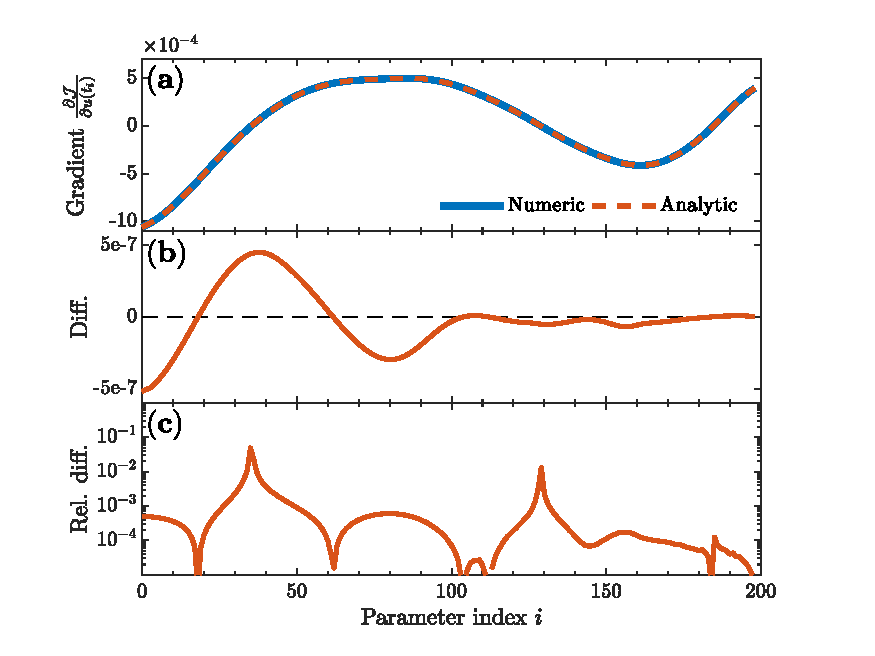
\includegraphics[width=0.8\textwidth]{Figures/CompareGradientsGRAPE.pdf}
    \caption{\textit{\textbf{(a)}: Numerical gradient along with gradient calculated via eq. \eqref{eq:STcostgrad}. \textbf{(b)}: Difference between the two gradients. \textbf{(c)}: Absolute relative difference between the two gradients.}}
    \label{fig:CompareGradientsGRAPE}
\end{figure}
A comparison between a numerically calculated gradient and the analytically derived gradient of eq. \eqref{eq:STcostgrad} can be seen in figure \ref{fig:CompareGradientsGRAPE}. As evident from the figure, the derived cost gradient is very accurate, which is necessary for an efficient optimization procedure. The difference between the two gradients is largest at the beginning of the sequence, due to the accumulated error from the time evolution of $\ket{\chi (0)}$, which is derived from two time evolutions over the entire duration.


\section{Interior Point Methods} \label{sec:IntPoint}

The GRAPE method formulates the control problem as the minimization of the cost function \eqref{eq:grapeCost} while providing the derivative of the cost with respect to the control functions \eqref{eq:costGradient}. Thus, the optimal control can be found using well established methods from mathematical optimization theory \cite{deFouquieres2011}. Generally, control problems are very hard to solve, as they are highly non-linear, have many control parameters (even when parametrized), and are often subjected to a series of constraints. An example of the latter can be seen when considering optimizations within the Bose-Hubbard model, as the model is valid only within the tight-binding limit \cite{manybodyBloch}. Thus, the control problem will be subject to the non-linear constraint
\begin{equation}
	 V_{0}^{\mathrm{min}} \leq c (u(t)) \leq V_{0}^{\mathrm{max}} \; ,
\end{equation}
where $c (u)$ is some constraint function dependent on the parameterization of the problem.\\
Interior point methods are currently considered some of the most powerful algorithms for large-scale non-linear programming \cite{wright}. The methods update the control parameters using the derivatives of the cost function via Newtons method, however, they differ from the standard Newton approach in many ways to accommodate constraints \cite{Karmarkar1984,Wachter2006}. Interior point methods approach the solution from within the feasible region as opposed to other methods like Nelder-Mead, hence the name \textit{interior}. In addition, they provide efficient performance while having better theoretical properties than the standard simplex method \cite{wright}.\\

In this section the simplest version of non-linear interior point method is derived, however, many variants of the method exists with respect to update strategies \cite{Byrd1997,Fiacco1990}, line searches \cite{Waltz2006,Wachter2005,Fletcher2002}, handling non-convexity \cite{Vanderbei1999} and more.\\
Consider the general minimization problem of some objective $f(x)$
\begin{subequations}	
 \begin{align}
	\min_{x } 			\quad & f(x) 			\\
	\text{subject to} 	\quad & g(x) = 0  		\\ 
						   	  & h(x) \geq 0 	\; ,
\end{align}
\label{eq:GeneralOptProblem}
\end{subequations}
where $g(x)$ and $h(x)$ are a set of equality and inequality constraints. The Lagrangian for the general constrained optimization problem \eqref{eq:GeneralOptProblem} is defined as
\begin{equation}
	\mathcal{L}(x,\lambda,\zeta) = f(x) - \lambda^T g(x) - \zeta^T h(x)  \; ,
\end{equation}
where $\lambda$ and $\zeta$ are vectors of Lagrange multipliers of the equality and inequality constraints respectively. Thus, one must find a point $(x^*,\lambda^*,\zeta^*)$ minimizing the objective function while satisfying the constraints.

\subsection{Duality}
Duality theory describes how an alternative \textit{dual} problem can be derived from the original \textit{primal} problem and how the two problems are related. Thus, the dual problem can be regarded as a different perspective of the original problem. Much information regarding the original problem can be inferred from the solution of its dual, hence many non-linear optimization algorithms solve primal-dual problems \cite{wright}.\\
The dual function is defined as
\begin{equation}
	q (\lambda , \zeta) = \inf_{x} \mathcal{L} (x,\lambda,\zeta) \; ,
\end{equation}
where the infimum is required to exist and be finite. Note how the Lagrange multipliers of the primal problem are the optimization parameters of its dual. The dual function always satisfies the condition of \textit{weak duality}
\begin{equation}
	f(x^*) \geq q (\lambda^* , \zeta^*) \; ,
	\label{eq:WeakDuality}
\end{equation} 
whereby it provides a lower bound on the solution of \eqref{eq:GeneralOptProblem}. In order for the direction of the inequality constraint to remain the same, it is necessary that all the inequality Lagrange multipliers fulfill $\zeta_i \geq 0$. This requirement can be considered a constraint of the dual, since the Lagrange multipliers are the variables of the dual function \cite{wright}. Thus, the dual problem is defined as
\begin{subequations}	
 \begin{align}
	\max_{\lambda , \zeta} 	\quad 	& q(\lambda , \zeta) 				\\
	\text{subject to} 		\quad 	& \zeta \geq 0  			\; .
\end{align}
\label{eq:GeneralDualProblem}
\end{subequations}
A very nice property of the dual problem is that it is always convex regardless of $f(x)$ \cite{Rockafellar1974}. Thus, the dual problem is often easier to solve than the primal. Furthermore, the solutions of the dual problem are the optimal Lagrange multipliers of the original problem, which would otherwise be very hard to find.
Another useful feature in duality theory is the \textit{duality gap}, which is given by the difference between the primal and dual function, $f(x) - q(\lambda , \zeta )$. Considering the condition of weak duality \eqref{eq:WeakDuality}, the duality gap implies that
\begin{equation}
	f(x) - f(x^*) \leq f(x) - g(\lambda , \zeta) \; ,
	\label{eq:DualityGapIneq}
\end{equation}
whereby $x$ is primal optimal and $\lambda , \zeta$ are dual optimal, if the duality gap is zero. Thus, eq. \eqref{eq:DualityGapIneq} can be used as a stopping criteria for optimization algorithms, as the duality gap will tend towards zero for $x \to x^*$ \cite{wright}.


\subsection{Karush–Kuhn–Tucker Conditions}
The Karush–Kuhn–Tucker (KKT) conditions are a set of first-order necessary conditions for a point $(x^*,\lambda^*,\zeta^*)$ being an optimum \cite{Kuhn2014}. They only consider properties of the gradient of the objective and constraint function, hence the \textit{first-order} label. The KKT conditions are very important in optimization theory, as many algorithms (including interior point methods) can be interpreted as solving a set of equations directly derived from the conditions \cite{wright}.    

\begin{theorem}
	Let the active constraints be all the equality constraints along with the set of inequality constraints fulfilling $h(x) = 0$ for some feasible $x$. Suppose that $x^*$ is a local solution of \eqref{eq:GeneralOptProblem} and the gradients of the active constraints are linearly independent at $x^*$. Then Lagrange multiplier vectors $\lambda$ and $\zeta$ exists, such that the following conditions are satisfied at $(x^*,\lambda^*,\zeta^*)$
\begin{subequations}	
\begin{align}
\nabla_x \mathcal{L}(x^*,\lambda^*,\zeta^*) &= 0 \; ,  	\\
g(x^*) &= 0 \; ,  \label{eq:KKTprimal1}					\\
h(x^*) &\geq 0 \; ,  \label{eq:KKTprimal2}				\\
\zeta^*  &\geq 0 \; , \label{eq:KKTdual}					\\ 
\zeta_{i}^* h_i (x^*) &= 0 \; , \quad \mathrm{for} \; i = 1 , \ldots , m \label{eq:KKTslack}
\end{align}
\label{eq:KKTconditions}
\end{subequations}	  
\end{theorem}
The first condition is called the \textit{stationary condition} and simply states that the point $(x^*,\lambda^*,\zeta^*)$ must be stationary point, which is a general requirement for a point to be considered an optimum. Next, the conditions \eqref{eq:KKTprimal1} and \eqref{eq:KKTprimal2} are the \textit{primal feasibility}, which coincide with the constraints originally stated in the problem \eqref{eq:GeneralOptProblem}. The following condition \eqref{eq:KKTdual} is the \textit{duality feasibility}, which is a constraint of the dual problem \eqref{eq:GeneralDualProblem} discussed earlier.
The last condition is the \textit{complementary slackness}, which arises from the requirement $\zeta^{*T} h(x^*) = 0$. The two previous conditions state that $\zeta_{i}^{*} h_i(x^*) \geq 0$, whereby the condition \eqref{eq:KKTslack} is needed for each inequality constraint.\\
If the point $(x^*,\lambda^*,\zeta^*)$ satisfies all the KKT conditions, then the point is the solution to the primal-dual problem.


\subsection{Basic Primal-Dual Interior Point Algorithm}
Interior point methods solve a set of equations derived directly from the KKT conditions using Newtons method. However, Newtons method is in general not compatible with inequality constraints, hence the original problem \eqref{eq:GeneralOptProblem} must be reformulated. Instead, the interior point methods solve barrier problems of the form 
\begin{subequations}	
 \begin{align}
	\min_{x,s} 			\quad & f(x) - \mu \sum_{i = 1}^{m} \log s_i \\
	\text{subject to} 	\quad & g(x) = 0  		\\ 
						   	  & h(x) - s  = 0 	\; ,
\end{align}
\label{eq:BarrierProblem}
\end{subequations}
where $\mu$ is the positive barrier parameter, and $s$ is a vector of slack variables, which transforms the inequality constraint into an equality at the cost of adding additional optimization variables. In order to ensure the direction of the inequality constraint, it is a requirement that $s \geq 0$. While this is an inequality constraint itself, it is enforced via the logarithmic barrier term, which diverges as any component of $s$ approaches zero. Furthermore, the barrier term does not add much complexity to the problem, as it convex and twice differentiable \cite{Wachter2006}.

The step direction towards the KKT-point can be found through Newtons method, however, often one can only take a small step before violating the constraints, hence the pure Newton direction is dubbed the \textit{affine scaling direction} \cite{wright}. The barrier approach consists of finding solutions of the barrier problem \eqref{eq:BarrierProblem} for a sequence of barrier parameters $\{ \mu_k \}$ converging to zero. Several strategies exist for updating the barrier parameters \cite{Byrd1997,Fiacco1990}, however, their common goal is to bias the step direction of the algorithm, such that the longest possible steps can be taken. The solutions of the barrier subproblems can be denoted $(x(\mu),s(\mu), \lambda(\mu),\zeta(\mu))$, and the trajectory of these points is known as the \textit{primal-dual central path}, which converges to $(x^*,s^*, \lambda^*,\zeta^*)$ as $\mu \to 0$ \cite{wright}.\\

The KKT conditions of the barrier problem \eqref{eq:BarrierProblem} can be expressed in a single mapping 
\begin{equation}
	F \equiv 
	\begin{bmatrix}
  \nabla_x f(x) - A_{g}^{T}(x) \lambda  - A_{h}^{T}(x) \zeta \\
  S \zeta - \mu e \\
  g(x)		\\
  h(x) - s 
  \end{bmatrix}
  = 0 \; ,
  \label{eq:BarrierKKTmap}
\end{equation}
where $A_g (x)$ and $A_h (x)$ are the Jacobian matrices of the constraint functions $g(x)$ and $h(x)$. Additionally, $S$ and $Z$ are defined as diagonal matrices with entries given by the vectors $s$ and $\zeta$, while $e = (1 ,1 , \ldots , 1 )^T$. Note how the introduction of the slack variables and the barrier term has modified the original KKT conditions \eqref{eq:KKTconditions}. Transforming the constraints has removed the need for the duality feasibility \eqref{eq:KKTdual}, while barrier term "relaxes" the complementary slackness \eqref{eq:KKTslack}, whose original form is recovered as $\mu \to 0$ \cite{wright}.\\
Applying Newtons method to the set of non-linear equations \eqref{eq:BarrierKKTmap} yields
\begin{equation}
  \begin{bmatrix}
  \nabla_{xx} \mathcal{L} 	& 0 	& -A_{g}^{T}(x)	& -A_{h}^{T}(x)	\\
  0 						& Z 	& 0 			& S 			\\
  A_{g}(x) 					& 0 	& 0 			& 0				\\
  A_{h}(x) 					& -I	& 0				& 0				 
  \end{bmatrix}  
  \begin{bmatrix}
  p_x \\ p_s \\ p_{\lambda} \\ p_{\zeta} 
  \end{bmatrix}
  = - F
  \label{eq:ConNewtonMethod}
\end{equation}
where $p = ( p_x , p_s , p_{\lambda} , p_{\zeta} )$ is the constrained Newton step direction, and $\mathcal{L}$ denotes the Lagrangian of the barrier problem \eqref{eq:BarrierProblem}
\begin{equation}
	\mathcal{L}(x,s,\lambda,\zeta) = f(x) - \lambda^T g(x) - \zeta^T ( h(x) - s)  \; .
\end{equation}
After computing the step, the parameters are iterated according to 
\begin{equation}
\begin{bmatrix}
  x^{k+1} \\ s^{k+1} \\ \lambda^{k+1} \\ \zeta^{k+1} 
\end{bmatrix} 
=
\begin{bmatrix}
  x^{k} \\ s^{k} \\ \lambda^{k} \\ \zeta^{k} 
\end{bmatrix} 
+ \alpha \circ p \; ,
\label{eq:ConNewtonStep}
\end{equation}
where $\alpha$ is a vector of step-sizes for each of the parameters. The step-size is commonly determined via a line-search \cite{Wachter2005,Fletcher2002}, although alternative methods exists \cite{Coleman1996}.\\
Interior point methods are capable of finding optimal solutions of non-linear constrained point using the methods described above, which can be summarized in the following algorithm \cite{wright}:
\begin{algorithm}
\begin{algorithmic}
\caption{Basic Primal-Dual Interior Point Algorithm}
\State Choose initial $\mu_0 > 0$.
\State Choose initial point $(x_0 , s_0 ,  \lambda_0 , \zeta_0)$.
\While{overall stopping criteria not met}
	\While{subproblem stopping criteria not met}
		\State Solve eq. \eqref{eq:ConNewtonMethod} to obtain search direction $p$.
		\State Compute step-size vector $\alpha$.
		\State Update $(x_k , s_k ,  \lambda_k , \zeta_k)$ according to eq. \eqref{eq:ConNewtonStep}.
	\EndWhile
	\State Update barrier parameter $\mu_k$.
\EndWhile
\end{algorithmic}
\end{algorithm}

\subsection{Implementation with GRAPE} \label{sec:IpoptGRAPE}
The interior point method is used here for minimizing the cost function \eqref{eq:grapeCost}, which is a function of a set of control parameters $u_n = \left( u_n (t_1) , \ldots , u_n (t_N)  \right)$. Examining the set of equations solved by the interior point method \eqref{eq:ConNewtonMethod} reveals that in order to compute the search direction, $p$, one needs the gradient of the objective function, $\nabla f(x)$, the Jacobian matrices of the constraints, $A_g (x)$ and $A_h (x)$, and finally the Hessian of both the objective and constraints contained in $\nabla_{xx} \mathcal{L}$.
The GRAPE method provides the gradient of the cost function through eq. \eqref{eq:costGradient}. 
Meanwhile, the constraints are dependent on the specific problem. In this case, the problem is crossing the phase transition between the superfluid and Mott-Insulator of the Bose-Hubbard model. As discussed in section \ref{sec:modTMDRG}, the control is parametrized as the interaction matrix element, $U$, which is directly dependent of the lattice depth as illustrated in figure \ref{fig:UJparameters}. Thus, the control problem is constrained by 
\begin{equation}
	U_{\mathrm{min}} \leq U(t_j) \; , \quad \mathrm{for} \; j = 1 , \ldots , N \; ,
	\label{eq:BoseHubbardConstraint}
\end{equation} 
for some $U_{\mathrm{min}}$ chosen such that the lattice depth is not below the tight binding limit, whereby the Bose-Hubbard model remains valid throughout the optimization \cite{manybodyBloch}. In the GRAPE parametrization the constraint function \eqref{eq:BoseHubbardConstraint} is the control itself, whereby the constraint Jacobian is simply the identity matrix. 
Furthermore, the second derivatives of the constraints completely vanish. Nevertheless, the Hessian of the cost function is still required in order to solve the equations \eqref{eq:ConNewtonMethod}. Although the second derivative of the cost function \eqref{eq:grapeCost} is analytically derivable (see Appendix \ref{chap:Hessian}), the numerical cost of computing the Hessian is rather high. Instead, Quasi-Newton methods can be used, where the Hessian can be approximated through various formulas \cite{wright}. The implementation of the interior point algorithm used in this thesis is from the IPOPT library \cite{Wachter2006}, which approximates the Hessian through the L-BFGS algorithm, which builds the matrix using the gradients of previous iterations \cite{Liu1989}. The combination of interior point methods and the GRAPE algorithm works really well in practice, as interior point methods attempt to solve the problem using as few steps as possible \cite{wright}, which is ideal, as the GRAPE gradient is very costly to compute.



\section{Control Parametrization via Chopped Basis} \label{sec:GROUP}
The convergence rate of gradient-based optimal control methods such as GRAPE have been shown to be much better than gradient-free methods for multiple problems \cite{Jager2014, sorensen2018}
One of the main disadvantages of GRAPE is the dimension for the optimization. As the duration of the control pulse is discretized into $N$ time-steps, the control value at each time slice, $u_n (t_j)$, is considered an optimization parameter. For long durations or small time-steps the resulting dimension of the optimization ($N$) will be very large. Thus, this type of control parametrization can be considered having too many degrees of freedom for the optimization.\\
Employing a proper parametrization of the control can drastically reduce the optimization dimension \cite{Winckel2008}.
A common choice is employing a chopped basis, which parametrizes the control as
\begin{equation}
	u(t) = u_0 (t) + S(t) \sum_{n=1}^{M} c_n f_n (t) \; , \label{eq:controlParametrization}
\end{equation}   
where $f_n$ are the basis functions, and $c_n$ are the optimization coefficients. In addition, $u_0 (t)$ is the initial control function, and $S (t)$ is a shape function enforcing the boundary conditions of the control, whereby $S(0) = S(T) = 0$ \cite{sorensen2018}. The shape function used throughout this thesis consists of two steep sigmoids oriented such that $S$ is unit for most time steps. The basis functions, $f_n$, must be chosen based on physical insight of the system \cite{Ruths2012}. For the control problem discussed in this thesis, employing a basis of sine functions has proven itself useful, as the sine functions are excellent at describing the smoothly varying control pulses desired \cite{sorensen2018,Jiang2009}. Thus, the basis functions read $f_n = \sin \left( \omega_n t / T \right)$, where $\omega_n = n \pi$ can be considered the Fourier components of the description.
An extension of this type of chopped basis was done in \cite{Doria2011,Caneva2011crab}, introducing random shifts to the frequencies resulting in the Chopped RAndom Basis or \textsc{CRAB}. In recent years the \textsc{CRAB} parametrization has been used together with the Nelder-Mead hill climbing algorithm to solve various control problems \cite{Doria2011,Caneva2011,FrankBloch,Lloyd2014}.\\
The great advantage of employing a reduced basis representation is the drastic reduction in the optimization space. However, artificial minima may be introduced, if the chosen basis is incapable of spanning the part of the optimization space containing the optimal solutions \cite{Rach2015}. Hence, the chopped basis dimension, $M$, must be chosen with consideration.


\subsection{Gradient-Optimization Using Parametrization - GROUP}
The Gradient-Optimization Using Parametrization or \textsc{GROUP} algorithm introduced in \cite{sorensen2018} combines the chopped basis representation with the \textsc{GRAPE} algorithm. A comparison between different optimization algorithms for optimal control demonstrated that \textsc{GROUP} outperformed both \textsc{GRAPE} and Nelder-Mead with \textsc{CRAB} in term of fidelity reached and number of function evaluations required for convergence. \\
Parameterizing the control alters the gradient of the cost function \eqref{eq:costGradient}. The new gradient can be derived using the chain rule
\begin{align}
	\frac{\partial \mathcal{J} (c)}{\partial c_n} &= \sum_{j = 1}^{N} \frac{\partial \mathcal{J} (u)}{\partial u(t_j)} \frac{\partial u(t_j)}{\partial c_n} \nonumber \\
	&= \sum_{j = 1}^{N} \frac{\partial \mathcal{J} }{\partial u(t_j)} S(t_j) f_n(t_j) \; , \label{eq:GROUPgradient} 
\end{align}
where only a single control has been chosen for cleaner notation. The gradient in \textsc{GROUP} is more complicated than in \textsc{GRAPE}, however, the cost of computing the gradient is still dominated by the evaluation of the original derivative ${\partial \mathcal{J} }/{\partial u(t_j)}$. Therefore, the increased computational cost of evaluating the gradient can be considered negligible \cite{sorensen2018}.\\
In addition, the chopped basis parameterization changes the derivatives of the constraints as well. Thus, the new constraint Jacobian can be derived using the chain rule as well
\begin{align}
	(A_h (c))_{i,n}  &= \sum_{j = 1}^{N} \frac{\partial h_i (u ) }{\partial u(t_j)} \frac{\partial u(t_j)}{\partial c_n} \nonumber \\
	&= \sum_{j = 1}^{N} (A_h (u))_{i,j} S(t_j) f_n (t_j) \; , \label{eq:GROUPconstJacobian} 
\end{align}
where $h(u)$ are the constraint functions, and $(A_h (u))_{i,j} = {\partial h_i (u ) } / {\partial u(t_j)}$ are recognized as the elements of the GRAPE parametrized constraint Jacobian. As discussed in section \ref{sec:IpoptGRAPE}, the constraint Jacobian is simply the identity matrix for the control problem treated here, whereby 
\begin{equation}
	(A_h (c))_{i,n} = \sum_{j = 1}^{N} \delta_{i,j} S(t_j) f_n (t_j) = S(t_i) f_n (t_i) \; .
\end{equation} 
Thus, the elements of the parametrized $N \times M$ Jacobian matrix remain constant throughout the entire optimization process for this problem.\\
Lastly, the parameterization of the control also alters the Hessians of the control problem. However, the implementation of the interior point method used here \cite{Wachter2006} is capable of approximating both the objective and constraint Hessians from previous derivatives using the L-BFGS algorithm \cite{Liu1989}. Therefore, calculating the transformed first-order derivatives is sufficient, and the general Hessians will not be derived here.


\section{Quantum Speed Limit}
A subtlety in the formulation of optimal control problems is that one is only searching for the control, $\boldsymbol{u}(t)$, which steers the initial state into the target-state at exactly the duration $t = T$. However, it is often desirable to obtain the desired state in the shortest timespan possible. If a solution exists at $t= T_1$, it might not exist at $t = T_2 < T_1$. The shortest duration for which a solution can be found is called the \textit{quantum speed limit} (QSL). The speed at which the system can evolve is determined by the relevant energy scales. If the system only has access to finite energies, a lower bound for how fast the system can evolve exists, which in turn leads to the QSL \cite{Caneva2009}.

The quantum speed limit can also be interpreted geometrically by examining how the state of the system moves through the Hilbert space. Considering the transfer $\ket{\psi} \to \ket{\chi}$, the fidelity $F = |\braket{\psi | \chi}|$ is a measure of the overlap of the states. The fidelity is zero if the two states are orthogonal, while its maximum value of one is obtained if the states are identical up to a global phase. The distance between the two states in the Hilbert space can be interpreted as an angle \cite{Wootters1981}
\begin{equation}
	\theta = \arccos \left( \sqrt{F} \right) \; ,
\end{equation}
where an angle of $\theta = \pi / 2 $ corresponds to orthogonal states, while states of unit fidelity are equivalent to $\theta = 0 $. The velocity of the state evolution can be defined as the rate of change of the angle, which is given by \cite{Aharonov}
\begin{equation}
	\dv{\theta}{t} = \Delta E \; ,
\end{equation}
where $\Delta E$ is the energy spread given by the variance of the Hamiltonian
\begin{equation}
	\Delta E  =  \sqrt{\Braket{\psi | \hat{H}^ 2 | \psi} - \Braket{\psi | \hat{H} | \psi} ^ 2 } \; .
\end{equation}
The energy spread must obey the Heisenberg time-energy uncertainty principle providing a fundamental limit to the velocity in the Hilbert space. The quantum speed limit for the transfer between two arbitrary states $\ket{\psi}$ and $\ket{\chi}$ separated by the angle $\theta$ was derived in \cite{Mandelstam1991} as
\begin{equation}
	T_{\mathrm{QSL}} = \frac{\theta}{\Delta E} \; . \label{eq:Mandelstam}
\end{equation}
However, the derivation of \eqref{eq:Mandelstam} assumes a time-independent Hamiltonian, which is very rarely the case in optimal control problems. The quantum speed limit for a time-dependent energy spread can be derived using arguments from differential geometry \cite{Aharonov,beyondQSL}
\begin{equation}
	\int_{0}^{T} \Delta E(t) \mathrm{d}t \geq \theta \; . \label{eq:HilbertPath}
\end{equation}
Eq. \eqref{eq:HilbertPath} states that the path length transversed in the Hilbert space is bounded by the initial angle $\theta$. The quantum speed limit is reached when the time-dependent Hamiltonian realizes the most direct path in the Hilbert space between the states $\ket{\psi}$ and $\ket{\chi}$. Note that eq. \eqref{eq:HilbertPath} does not directly provide the quantum speed limit, as the control functions corresponding to the shortest path are not known in general. The presence of a phase transition further complicated the problem, as the rate at which information is spread within the system is bounded by the effective light cone resulting from the local Hamiltonian.
Hence, determining the quantum speed limit is often considered an optimization problem in itself.

The quantum speed limit can be extracted from an optimal solution by examining the relative motion of $\ket{\psi (t)}$ in the Hilbert space. Assuming the state is evolved according the optimal Hamiltonian realizing the equality of eq. \eqref{eq:HilbertPath}. Thus, the direct velocity in the Hilbert space is given by $Q_{\mathrm{opt}} (t) = \Delta E_{\mathrm{opt}}(t)$, and the obtained fidelity can be expressed as a function of duration \cite{beyondQSL}
\begin{equation}
	F(T) = \sin ^2 \left( \int_{0}^{T} Q_{\mathrm{opt}} (t) \mathrm{d} t \right) \; ,
	\label{eq:FidelityDurationSin1}
\end{equation}  
if the states $\ket{\psi}$ and $\ket{\chi}$ are orthogonal. Interpreting the state as moving along a geodesic in the Hilbert space between the two orthogonal states, the direct velocity is given by $Q_{\mathrm{opt}} (t) =  -\dv{\theta (t)}{t}$, whereby
\begin{equation}
	F(T) = \sin ^2 \left( \int_{0}^{T} - \dv{\theta (t)}{t} \mathrm{d} t \right) =  \sin ^2 \left( \eval{ - \theta(t)}_{0}^{T} \right) = \sin ^2 \left( \frac{\pi}{2} \frac{T}{T_{\mathrm{QSL}}} \right) \; .
	\label{eq:FidelityDurationSin2}
\end{equation}  
The relation $\theta (T) = \frac{\pi}{2} \left( 1 -  \frac{T}{T_{\mathrm{QSL}}} \right)$ is only valid if the state is moving on a geodesic, whereas eq. \eqref{eq:FidelityDurationSin1} is more general. A similar behavior to eq. \eqref{eq:FidelityDurationSin2} was reported in \cite{Caneva2011}, where a number of systems were shown to behave according to the relation. However, it should be stressed that the relation \eqref{eq:FidelityDurationSin2} requires the initial and final states to be orthogonal and the system to be recast as an effective two-level system.

For an example of optimal control see Appendix \ref{chap:LZexample}, which illustrates some of the consequences of the quantum speed limit.
